\documentclass{article}

\usepackage[utf8]{inputenc}
\usepackage[russian]{babel}
\usepackage[a4paper, margin=1in]{geometry}
\usepackage{graphicx}
\usepackage{amsmath}
\usepackage{wrapfig}
\usepackage{multirow}
\usepackage{mathtools}
\usepackage{pgfplots}
\usepackage{pgfplotstable}
\usepackage{setspace}
\usepackage{changepage}
\usepackage{caption}
\usepackage{csquotes}
\usepackage{hyperref}
\usepackage{listings}

\pgfplotsset{compat=1.18}
\hypersetup{
  colorlinks = true,
  linkcolor  = blue,
  filecolor  = magenta,      
  urlcolor   = darkgray,
  pdftitle   = {
    math-tool-report-approx-smirnov-victor-p32131
  },
}

\definecolor{codegreen}{rgb}{0,0.6,0}
\definecolor{codegray}{rgb}{0.5,0.5,0.5}
\definecolor{codepurple}{rgb}{0.58,0,0.82}
\definecolor{backcolour}{rgb}{0.99,0.99,0.99}

\lstdefinestyle{codestyle}{
  backgroundcolor=\color{backcolour},   
  commentstyle=\color{codegreen},
  keywordstyle=\color{magenta},
  numberstyle=\tiny\color{codegray},
  stringstyle=\color{codepurple},
  basicstyle=\ttfamily\footnotesize,
  breakatwhitespace=false,         
  breaklines=true,                 
  captionpos=b,                    
  keepspaces=true,                 
  numbers=left,                    
  numbersep=5pt,                  
  showspaces=false,                
  showstringspaces=false,
  showtabs=false,                  
  tabsize=2
}

\lstset{style=codestyle}

\begin{document}

\begin{titlepage}
    \begin{center}
        \begin{spacing}{1.4}
            \large{Университет ИТМО} \\
            \large{Факультет программной инженерии и компьютерной техники} \\
        \end{spacing}
        \vfill
        \textbf{
            \huge{Вычислительная математика.} \\
            \huge{Лабораторная работа №4.} \\
            \huge{Аппроксимация функций методом наименьших квадратов} \\
        }
    \end{center}
    \vfill
    \begin{center}
        \begin{tabular}{r l}
            Группа:  & P32131                  \\
            Студент: & Смирнов Виктор Игоревич \\
            Вариант: & 16                      \\
        \end{tabular}
    \end{center}
    \vfill
    \begin{center}
        \begin{large}
            2023
        \end{large}
    \end{center}
\end{titlepage}

\section*{Ключевые слова}
Интерполяция, Многочлен Лагранжа, Многочлен Ньютона.

\section{Цель работы}

Цель работы - решить задачу интерполяции, найти значения функции
при заданных значениях аргумента, отличных от узловых точек,
используя методы Лагранжа и Гаусса.

\section{Вычислительная задача}

\subsection{Описание}

Поставлена была ответственная задача: даны узлы интерполяции,
даны точки, значения многочлена в которых нужно интерполировать.
Для решения поставленной задачи воспользуемся библиотеками
уже родными библиотеками Mathematica и Sematica, разработанными
мною в процессе прохождения курса вычислительной математики в
Университете ИТМО (исходный код: \url{https://github.com/vityaman-edu/math-tool}).

\subsection{Программа для исследования}

\lstinputlisting[
    language={C++},
    caption={Тест для решения вычислительной задачи},
]{../../../test/Mathematica/Functional/Interpolation/Playground.cpp}

\subsection{Результаты измерений}

Посмотрим на результаты:

\begin{lstlisting}[
    language={Bash},
    caption={Результаты решения поставленной задачи  (коэффициенты были обрезаны до 2 знаков после запятой)},
]
Interpolation::symbolicLagrange:
(((((((0 + ((((((1.25 * ((x - 0.30) / -0.05)) * ((x - 0.35) / -0.10)) * ((x - 0.40) / -0.15)) * ((x - 0.45) / -0.20)) * ((x - 0.50) / -0.25)) * ((x - 0.55) / -0.30))) + ((((((2.17 * ((x - 0.25) / 0.05)) * ((x - 0.35) / -0.05)) * ((x - 0.40) / -0.10)) * ((x - 0.45) / -0.15)) * ((x - 0.50) / -0.20)) * ((x - 0.55) / -0.25))) + ((((((3.12 * ((x - 0.25) / 0.10)) * ((x - 0.30) / 0.05)) * ((x - 0.40) / -0.05)) * ((x - 0.45) / -0.10)) * ((x - 0.50) / -0.15)) * ((x - 0.55) / -0.20))) + ((((((4.04 * ((x - 0.25) / 0.15)) * ((x - 0.30) / 0.10)) * ((x - 0.35) / 0.05)) * ((x - 0.45) / -0.05)) * ((x - 0.50) / -0.10)) * ((x - 0.55) / -0.15))) + ((((((5.98 * ((x - 0.25) / 0.20)) * ((x - 0.30) / 0.15)) * ((x - 0.35) / 0.10)) * ((x - 0.40) / 0.05)) * ((x - 0.50) / -0.05)) * ((x - 0.55) / -0.10))) + ((((((6.91 * ((x - 0.25) / 0.25)) * ((x - 0.30) / 0.20)) * ((x - 0.35) / 0.15)) * ((x - 0.40) / 0.10)) * ((x - 0.45) / 0.05)) * ((x - 0.55) / -0.05))) + ((((((7.83 * ((x - 0.25) / 0.30)) * ((x - 0.30) / 0.25)) * ((x - 0.35) / 0.20)) * ((x - 0.40) / 0.15)) * ((x - 0.45) / 0.10)) * ((x - 0.50) / 0.05)))

Interpolation::symbolicNewton:
(((((((0 + (1.25 * 1)) + (18.41 * (1 * (x - 0.25)))) + (4.94 * ((1 * (x - 0.25)) * (x - 0.30)))) + (-58.26 * (((1 * (x - 0.25)) * (x - 0.30)) * (x - 0.35)))) + (7170.66 * ((((1 * (x - 0.25)) * (x - 0.30)) * (x - 0.35)) * (x - 0.40)))) + (-110072.00 * (((((1 * (x - 0.25)) * (x - 0.30)) * (x - 0.35)) * (x - 0.40)) * (x - 0.45)))) + (905928.88 * ((((((1 * (x - 0.25)) * (x - 0.30)) * (x - 0.35)) * (x - 0.40)) * (x - 0.45)) * (x - 0.50))))
Interpolation::Newton::dividedDifferences: 
0: 1.2557
1: 18.414
2: 4.94
3: -58.2667
4: 7170.67
5: -110072
6: 905929
lagrange(0.251) = 1.22013
newton(0.251) = 1.22013
lagrange(0.512) = 6.85843
newton(0.512) = 6.85843
lagrange(0.255) = 1.12252
newton(0.255) = 1.12252
lagrange(0.534) = 6.93994
newton(0.534) = 6.93994
lagrange(0.272) = 1.26425
newton(0.272) = 1.26425
lagrange(0.551) = 7.93733
newton(0.551) = 7.93733
lagrange(0.294) = 1.97998
newton(0.294) = 1.97998
lagrange(0.402) = 4.1112
newton(0.402) = 4.1112
lagrange(0.372) = 3.40014
newton(0.372) = 3.40014
lagrange(0.405) = 4.20971
newton(0.405) = 4.20971
lagrange(0.384) = 3.62562
newton(0.384) = 3.62562
lagrange(0.445) = 5.79299
newton(0.445) = 5.79299
lagrange(0.351) = 3.13273
newton(0.351) = 3.13273
lagrange(0.437) = 5.46635
newton(0.437) = 5.46635
\end{lstlisting}

\subsection{Анализ результатов}

Изобразим графики построенных многочленов.
Получается, что Лагранж и Ньютон построили
одинаковые многочлены.

\begin{figure}[h]
    \centering
    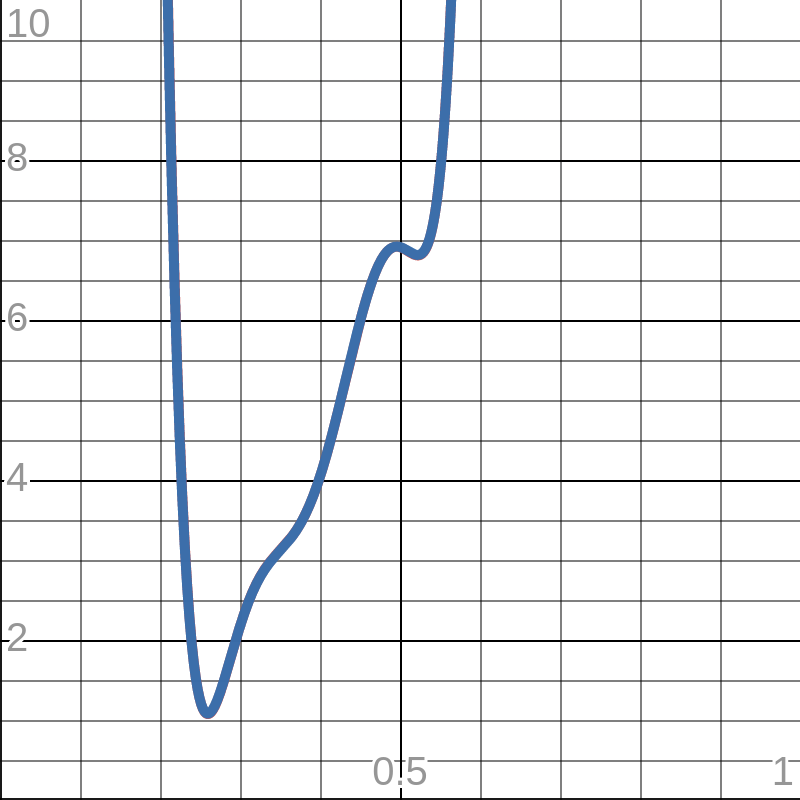
\includegraphics[totalheight=8cm]{graph.png}
    \caption{График построенного многочлена}
\end{figure}

\section{Программная реализация задачи}

\subsection{Метод Лагранжа}

\lstinputlisting[
    language={C++},
    caption={Метод Лагранжа},
    linerange={28-47}
]{../../../src/Mathematica/Functional/Interpolation/Lagrange.hpp}

\subsection{Метод Ньютона}

\lstinputlisting[
    language={C++},
    caption={Метод Ньютона},
    linerange={31-62},
]{../../../src/Mathematica/Functional/Interpolation/Newton.hpp}

\section{Вывод}

Выполнив данную лабораторную работу я познакомился
с базовыми методами построения интерполяционных 
многочленов. В отличие от задачи аппроксимации, 
интерполяция требует точного совпадения значений
многочлена в заданных точках, но ничего особо не 
говорит про значения в других точках. Хотя
на практике получается, что интерполяционные 
многочлены очень даже неплохо приближают функцию,
однако при небольших степенях. На данном их свойстве
основан метод интерполяции функции сплайнами: 
при таком подходе мы делим область определения 
функции на отрезки, на каждом отрезке интерполируем
ее многочленом (часто степени 3), а потом кусочно
задаем интерполяционную функцию, склеивая многочлены.

\begin{thebibliography}{9}

    \bibitem{calc-math-demidovich-maron}
    Б.П. Демидович, И.А. Марон Основы вычислительной математики:
    учебное пособие — 1966 год.

    \bibitem{itmo-lecture}
    Лекции Татьяны Алексеевны Малышевой

\end{thebibliography}

\end{document}
